% Compilare (din folderul licenta/):
%   pdflatex prezentare-5min.tex   (de doua ori pentru numerotare)
%
% Imagini: folderul images/ din lucrarea de diploma.
% Pentru slide-ul cu emotii, pune (optional) in images/:
%   emotie-happy.jpg  emotie-sad.jpg  emotie-surprised.jpg  emotie-angry.jpg
% (meltdown foloseste deja robot-meltdown-frontal.png). Daca lipsesc, apar
% automat casete-substitut, deci prezentarea compileaza oricum.

\documentclass[aspectratio=169,11pt]{beamer}

\usetheme{Madrid}
\usecolortheme{whale}
\usefonttheme{structurebold}
\setbeamertemplate{navigation symbols}{}
\setbeamertemplate{itemize items}[circle]

\usepackage[utf8]{inputenc}
\usepackage[T1]{fontenc}
\usepackage[romanian]{babel}
\usepackage{graphicx}
\usepackage{booktabs}
\usepackage{tikz}
\usetikzlibrary{positioning, arrows.meta, fit, backgrounds}

\graphicspath{{images/}}

\definecolor{fmiBlue}{RGB}{0,62,126}
\definecolor{fmiLight}{RGB}{232,241,250}
\definecolor{accentTeal}{RGB}{0,128,128}
\definecolor{softGray}{RGB}{120,130,140}

\setbeamercolor{structure}{fg=fmiBlue}
\setbeamercolor{block title}{bg=fmiBlue, fg=white}
\setbeamercolor{block body}{bg=fmiLight}
\setbeamercolor{block title alerted}{bg=accentTeal, fg=white}
\setbeamercolor{block body alerted}{bg=accentTeal!12}
\setbeamercolor{alerted text}{fg=accentTeal}
\setbeamerfont{block title}{size=\small}

% Footline compact cu titlu scurt + numar slide
\setbeamertemplate{footline}{%
  \leavevmode%
  \hbox{%
    \begin{beamercolorbox}[wd=.5\paperwidth,ht=2.4ex,dp=1ex,leftskip=1em]{author in head/foot}%
      \scriptsize TriSense — robotica asistiva
    \end{beamercolorbox}%
    \begin{beamercolorbox}[wd=.5\paperwidth,ht=2.4ex,dp=1ex,rightskip=1em]{title in head/foot}%
      \hfill\scriptsize\insertframenumber\,/\,\inserttotalframenumber
    \end{beamercolorbox}}%
  \vskip0pt}

\title{TriSense}
\subtitle{Sistem cyber-fizic adaptiv pentru robotica asistivă\\în intervenții pentru copii neurodivergenți}
\author{Boca Bogdan-Nicolae}
\institute{Facultatea de Matematică și Informatică\\Universitatea din București · Tehnologia Informației\\Coordonator: Lect. Dr. Anca Dobrovăț}
\date{iunie 2026}

% --- Diagrama arhitecturii (3 niveluri) ---
\newcommand{\triarch}{%
  \centering
  \resizebox{0.96\linewidth}{!}{%
  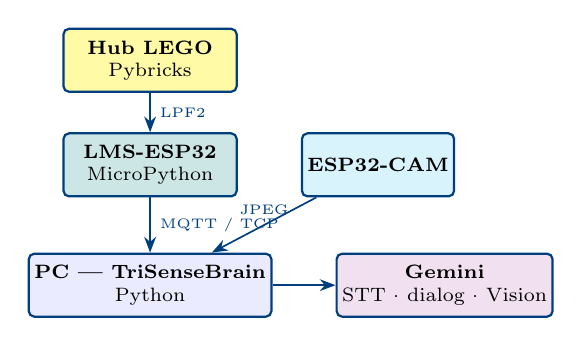
\begin{tikzpicture}[
    font=\scriptsize,
    box/.style={draw=fmiBlue, thick, rounded corners=2pt, align=center,
                minimum height=8mm, inner sep=2pt, fill=white},
    arr/.style={-{Stealth[length=2mm]}, semithick, fmiBlue},
  ]
    \node[box, fill=yellow!35, minimum width=22mm] (hub) {\textbf{Hub LEGO}\\Pybricks};
    \node[box, fill=teal!20, minimum width=22mm, below=5mm of hub] (esp) {\textbf{LMS-ESP32}\\MicroPython};
    \node[box, fill=cyan!15, minimum width=18mm, right=8mm of esp] (cam) {\textbf{ESP32-CAM}};
    \node[box, fill=blue!8, minimum width=24mm, below=7mm of esp] (pc) {\textbf{PC — TriSenseBrain}\\Python};
    \node[box, fill=violet!12, minimum width=20mm, right=8mm of pc] (cloud) {\textbf{Gemini}\\STT · dialog · Vision};
    \draw[arr] (hub) -- node[right, font=\tiny]{LPF2} (esp);
    \draw[arr] (esp) -- node[right, font=\tiny]{MQTT / TCP} (pc);
    \draw[arr] (cam) -- node[above, font=\tiny]{JPEG} (pc);
    \draw[arr] (pc) -- (cloud);
  \end{tikzpicture}}%
}

% --- Lant vocal (flux), in limbaj uman ---
\newcommand{\voicechain}{%
  \centering
  \resizebox{\linewidth}{!}{%
  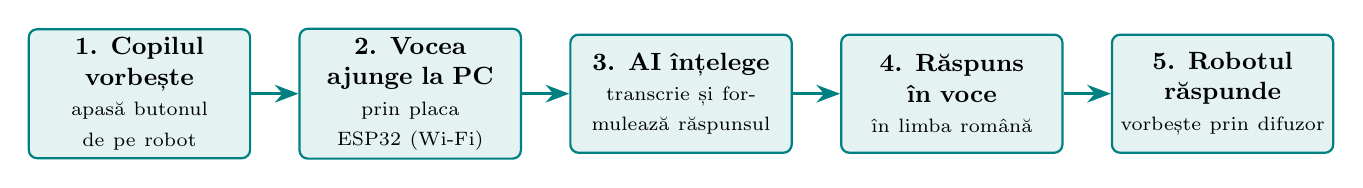
\begin{tikzpicture}[
    font=\small,
    s/.style={draw=accentTeal, thick, rounded corners=3pt, fill=accentTeal!10,
              align=center, minimum height=15mm, text width=26mm, inner sep=3pt},
    a/.style={-{Stealth[length=3mm]}, line width=1pt, accentTeal},
  ]
    \node[s] (mic) {\textbf{1. Copilul vorbește}\\{\scriptsize apasă butonul de pe robot}};
    \node[s, right=6mm of mic] (pc) {\textbf{2. Vocea ajunge la PC}\\{\scriptsize prin placa ESP32 (Wi-Fi)}};
    \node[s, right=6mm of pc] (ai) {\textbf{3. AI înțelege}\\{\scriptsize transcrie și formulează răspunsul}};
    \node[s, right=6mm of ai] (tts) {\textbf{4. Răspuns în voce}\\{\scriptsize în limba română}};
    \node[s, right=6mm of tts] (spk) {\textbf{5. Robotul răspunde}\\{\scriptsize vorbește prin difuzor}};
    \draw[a] (mic) -- (pc);
    \draw[a] (pc) -- (ai);
    \draw[a] (ai) -- (tts);
    \draw[a] (tts) -- (spk);
  \end{tikzpicture}}%
}

% --- Caseta pentru o emotie: poza daca exista, altfel substitut ---
\newcommand{\emocard}[2]{% #1 = fisier (fara extensie cautam .jpg/.png), #2 = eticheta
  \begin{minipage}[t]{0.185\textwidth}
    \centering
    \IfFileExists{images/#1.jpg}{%
      \includegraphics[width=\linewidth, height=2.2cm, keepaspectratio]{#1.jpg}%
    }{%
      \IfFileExists{images/#1.png}{%
        \includegraphics[width=\linewidth, height=2.2cm, keepaspectratio]{#1.png}%
      }{%
        \fbox{\begin{minipage}[t][2.2cm][c]{0.92\linewidth}\centering
          \scriptsize\color{softGray} foto\\ lipsă
        \end{minipage}}%
      }%
    }\\[2pt]
    {\scriptsize\textbf{#2}}
  \end{minipage}%
}

\begin{document}

% ===========================================================================
\begin{frame}[plain]
  \begin{columns}[c]
    \column{0.15\textwidth}
    
\includegraphics[width=\linewidth]{logo-ub.png}
    \column{0.7\textwidth}
    \centering
    {\usebeamerfont{title}\usebeamercolor[fg]{title}\inserttitle\par}
    \vspace{0.2em}
    {\color{fmiBlue}\rule{0.5\linewidth}{1pt}}\par
    \vspace{0.35em}
    {\usebeamerfont{subtitle}\insertsubtitle\par}
    \vspace{1.1em}
    {\large\insertauthor\par}
    \vspace{0.4em}
    {\small\insertinstitute\par}
    \vspace{0.6em}
    {\small București, \insertdate\par}
    \column{0.15\textwidth}
    
\includegraphics[width=\linewidth]{logo-fmi.png}
  \end{columns}
\end{frame}

% ===========================================================================
\begin{frame}{De ce această temă?}
  \begin{columns}[T]
    \column{0.55\textwidth}
    \begin{block}{Context și motivație}
      \begin{itemize}
        \item Spectru autist și ADHD — nevoie mare de intervenții timpurii; în România, resurse limitate.
        \item \textbf{LEGO-Based Therapy} (LeGoff): mediu predictibil, colaborare fără ambiguitate socială.
        \item \textbf{Robotica asistivă:} robotul ca \emph{mediator}, nu înlocuitor al terapeutului.
      \end{itemize}
    \end{block}
    \begin{alertblock}{Punctul de plecare}
      Putem integra LEGO educațional + ESP32 + laptop într-un robot cu dialog vocal, jocuri structurate și metrici pentru terapeut?
    \end{alertblock}
    \column{0.42\textwidth}
    \centering
    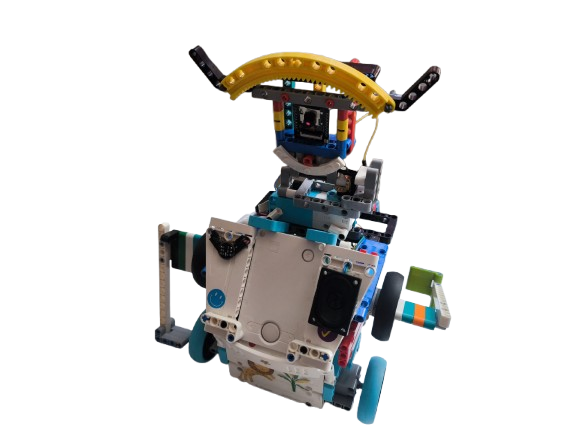
\includegraphics[width=0.96\linewidth]{robot-trisense-perspectiva.png}\\[2pt]
    {\scriptsize Prototipul TriSense — LEGO SPIKE Prime + LMS-ESP32}
  \end{columns}
\end{frame}

% ===========================================================================
\begin{frame}{Structura lucrării scrise}
  \begin{columns}[T]
    \column{0.62\textwidth}
    \begin{enumerate}
      \item \textbf{Introducere} — context, problemă, obiective și contribuții
      \item \textbf{Preliminarii} — fundamente teoretice (LBT, robotică asistivă, cadre psihologice)
      \item \textbf{Arhitectura sistemului} — cele 3 niveluri, protocoale, fluxuri de date
      \item \textbf{Implementare} — firmware, creierul PC, jocuri, vedere artificială
      \item \textbf{Evaluare} — testare, rezultate, considerații etice
      \item \textbf{Concluzii} — sinteză și direcții de dezvoltare
    \end{enumerate}
    \vspace{0.3em}
    {\scriptsize Materialul detaliat (catalogul jocurilor, listările de cod, figurile) este reluat în Anexe.}
    \column{0.36\textwidth}
    \centering
    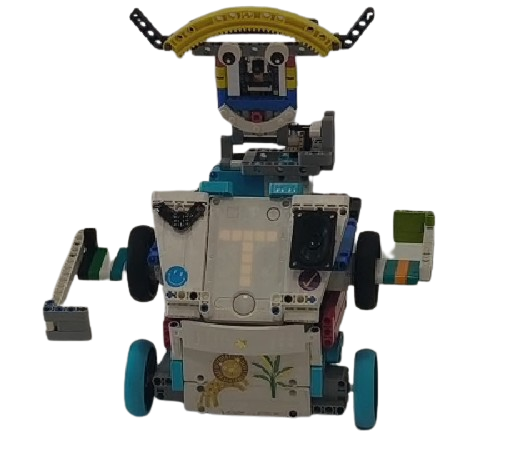
\includegraphics[width=0.96\linewidth]{robot-trisense.png}\\[2pt]
    {\scriptsize Robotul TriSense}
  \end{columns}
\end{frame}

% ===========================================================================
\begin{frame}{Problema și scopul}
  \begin{columns}[T]
    \column{0.52\textwidth}
    \begin{alertblock}{Provocarea}
      Să faci să lucreze împreună, în timp real, un robot LEGO care singur nu se poate conecta la rețea, o plăcuță care îi dă Wi-Fi, o cameră și inteligența artificială din cloud — fără ca robotul să se blocheze sau să devină imprevizibil în fața copilului.
    \end{alertblock}
    \begin{block}{Ce vreau să ofere}
      \begin{itemize}
        \item jocuri terapeutice ghidate;
        \item dialog cu robotul, în limba română;
        \item verificarea construcțiilor LEGO cu camera;
        \item \textbf{rapoarte de sesiune} pentru terapeut.
      \end{itemize}
    \end{block}
    \column{0.46\textwidth}
    \begin{block}{Ce am realizat}
      \small
      \begin{itemize}
        \item un sistem împărțit pe 3 niveluri, ușor de testat;
        \item dialog vocal complet (copilul vorbește, robotul răspunde);
        \item butoanele robotului ca mod de interacțiune;
        \item robotul „vede” construcțiile fără antrenament prealabil;
        \item peste 10 activități + raport automat de sesiune.
      \end{itemize}
    \end{block}
    {\scriptsize Testat pe robotul real; cu sprijinul psihoterapeuților Lumpan (terapie LEGO, România).}
  \end{columns}
\end{frame}

% ===========================================================================
\begin{frame}{Cum e construit sistemul}
  \begin{columns}[T]
    \column{0.42\textwidth}
    \triarch
    \vspace{0.4em}

    {\footnotesize Fiecare parte face ce știe cel mai bine: robotul LEGO se mișcă (dar nu are Wi-Fi), placa ESP32 îi dă legătura la rețea, iar PC-ul gândește.}
    \column{0.56\textwidth}
    \small
    \begin{block}{Ce vede și aude copilul}
      Robotul LEGO (brațe, roți, ecran cu lumini, butoane), microfonul și difuzorul de pe placa ESP32 și o cameră (ESP32-CAM) care îi fotografiază construcțiile.
    \end{block}
    \begin{block}{„Creierul” de pe calculator}
      \textbf{Python} — coordonează totul: jocurile, dialogul, metricile.\\
      \textbf{Google Gemini} — înțelege vorbirea, poartă conversația și „se uită” la construcțiile LEGO.\\
      \textbf{Sinteză vocală} în limba română.
    \end{block}
    \begin{block}{Cum comunică între ele}
      Mesaje scurte de comandă (MQTT), legătura robot–placă (LPF2) și sunetul în timp real (TCP).
    \end{block}
  \end{columns}
\end{frame}

% ===========================================================================
\begin{frame}{Cum circulă vocea — pas cu pas}
  \vspace{0.6em}
  \voicechain
  \vspace{1.0em}

  \centering
  {\small Totul rulează pe componente ieftine, ușor de procurat. Partea grea nu e o piesă scumpă, ci felul în care toate lucrează împreună fără întreruperi — exact ce contează când în fața robotului stă un copil.}
\end{frame}

% ===========================================================================
\begin{frame}{Cablajul electric}
  \centering
  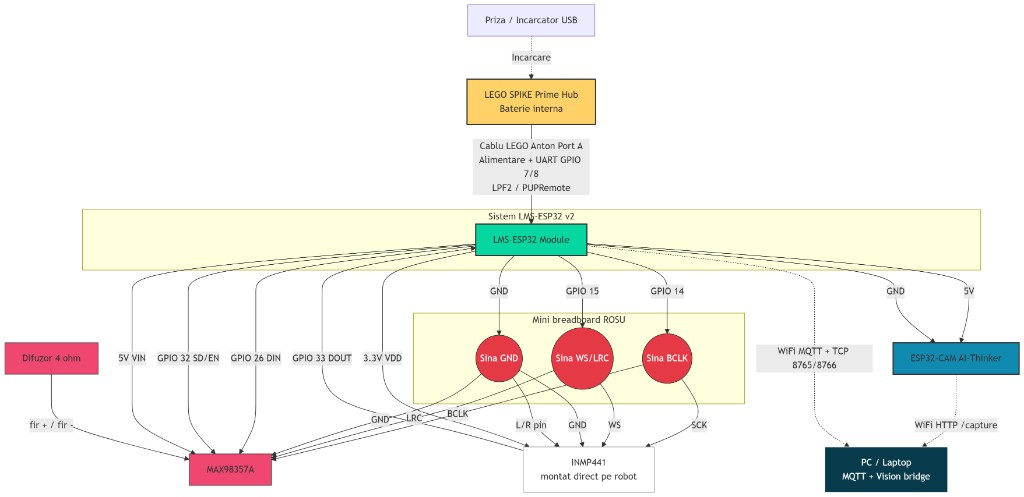
\includegraphics[height=0.78\textheight, keepaspectratio]{cablaj-trisense.png}\\[4pt]
  {\scriptsize Conexiunile fizice: placa ESP32, amplificatorul audio, difuzorul și camera ESP32-CAM}
\end{frame}

% ===========================================================================
\begin{frame}{Funcționalități terapeutice}
  \begin{columns}[T]
    \column{0.58\textwidth}
    \small
    \begin{table}
      \begin{tabular}{@{}p{3.5cm}p{4.2cm}@{}}
        \toprule
        \textbf{Activitate} & \textbf{Construct vizat} \\
        \midrule
        Ghicește emoția & etichetarea emoțiilor \\
        Urmează tiparul & imitație, memorie secvențială \\
        Build the Model + CAM & planificare vizuo-spațială \\
        Stop \& Go, timp, categorii & funcții executive \\
        Poveste co-construită & narativă, schimb de rând \\
        Respirație, dans & autoreglare, descărcare \\
        \bottomrule
      \end{tabular}
    \end{table}
    \textbf{Infrastructură:} metrici CSV/JSONL · raport \texttt{session\_reports/}\\
    \textit{\scriptsize Datele susțin joc ghidat, nu diagnostic clinic.}
    \column{0.40\textwidth}
    \centering
    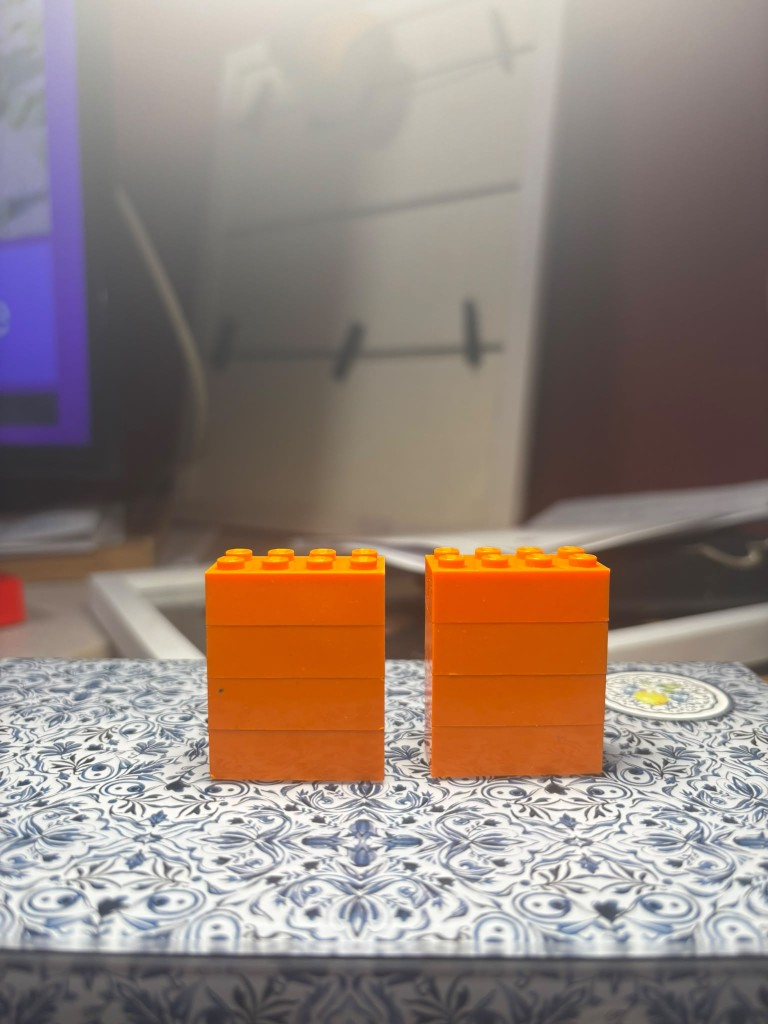
\includegraphics[width=0.32\linewidth]{build-model-nivel1.png}\hfill
    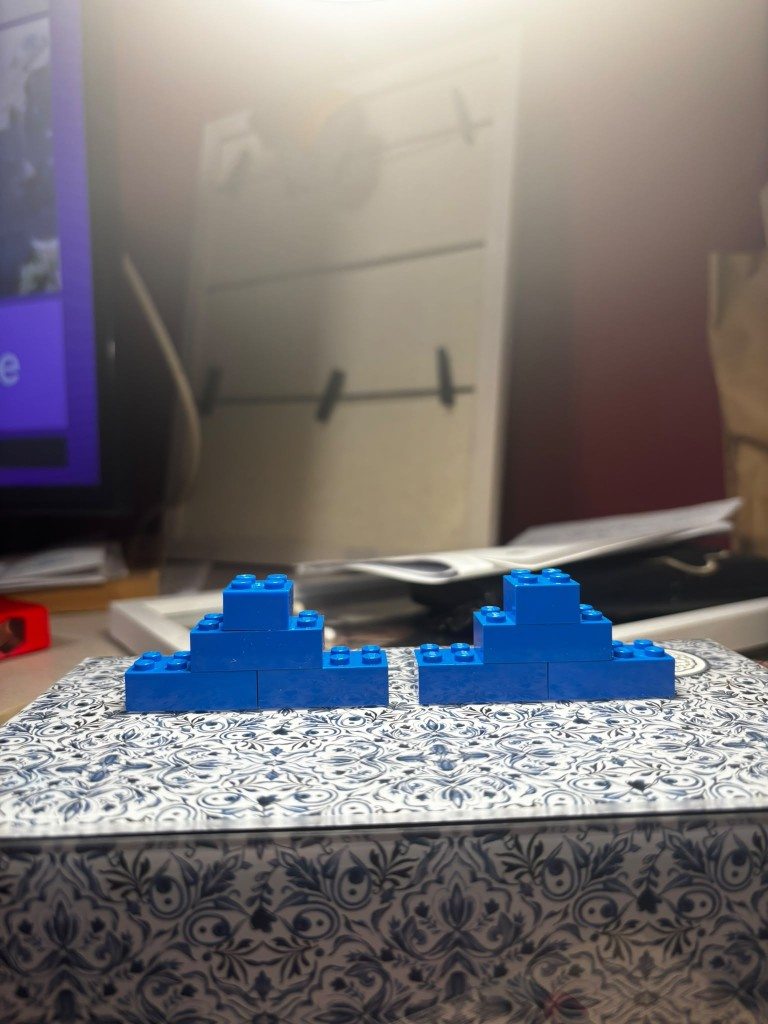
\includegraphics[width=0.32\linewidth]{build-model-nivel2.png}\hfill
    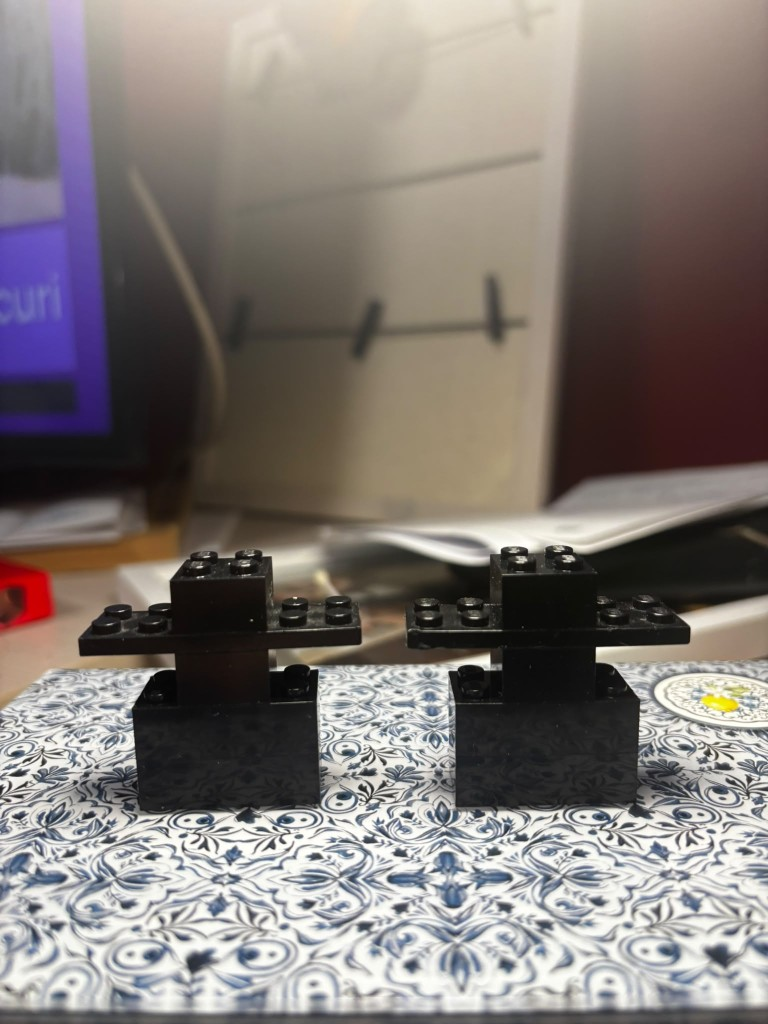
\includegraphics[width=0.32\linewidth]{build-model-nivel3.png}\\[2pt]
    {\scriptsize Build the Model — 3 nivele}\\[6pt]
    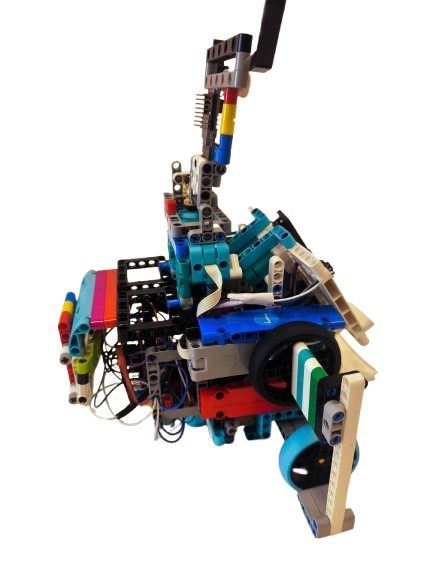
\includegraphics[width=0.92\linewidth]{robot-trisense-lateral.png}\\[2pt]
    {\scriptsize Verificare LEGO: ESP32-CAM + Gemini Vision}
  \end{columns}
\end{frame}

% ===========================================================================
\begin{frame}{„Ghicește emoția” — cele 5 emoții}
  \centering
  Robotul arată o emoție prin mișcare, lumini și sunet; copilul o numește.
  \vspace{0.8em}

  \emocard{emotie-happy}{Fericit}\hfill
  \emocard{emotie-sad}{Trist}\hfill
  \emocard{emotie-surprised}{Surprins}\hfill
  \emocard{emotie-angry}{Furios}\hfill
  \emocard{robot-meltdown-frontal}{Criză (meltdown)}

  \vspace{0.9em}
  {\footnotesize Fiecare emoție = o combinație de gesturi (brațe/roți), expresie pe matricea LED și ton vocal.}
\end{frame}

% ===========================================================================
\begin{frame}{Concluzii și direcții viitoare}
  \begin{columns}[T]
    \column{0.5\textwidth}
    \begin{block}{Concluzii}
      \begin{itemize}
        \item Sistem funcțional \textbf{cap-coadă} pe hardware real.
        \item Arhitectura pe 3 niveluri = cheia integrării și a testării izolate.
        \item Componente \textbf{accesibile}; diferența o face integrarea, replicabilă oriunde.
      \end{itemize}
    \end{block}
    \column{0.5\textwidth}
    \begin{block}{Direcții viitoare}
      \begin{itemize}
        \item validare clinică extinsă, cu terapeuți;
        \item detecția emoției din voce (prozodie);
        \item detecție automată a vorbirii (VAD);
        \item funcționare offline (modele locale);
        \item interfață web pentru terapeut.
      \end{itemize}
    \end{block}
  \end{columns}
\end{frame}

% ===========================================================================
\begin{frame}[plain,c]
  \centering
  \vspace{0.5em}
  {\usebeamerfont{title}\color{fmiBlue}Vă mulțumesc!}\\[0.4em]
  {\large Întrebări \& Răspunsuri}\\[0.8em]
  {\Large $\rightarrow$ \textbf{Demonstrație live — TriSense}}\\[0.9em]
  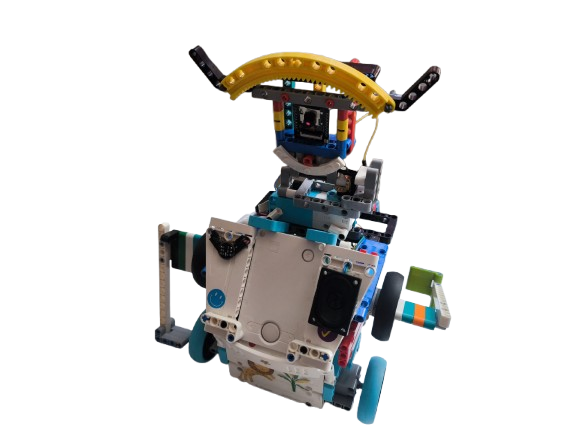
\includegraphics[width=0.36\textwidth]{robot-trisense-perspectiva.png}\\[0.7em]
  {\small
    Dialog vocal · jocuri terapeutice · construcții LEGO · metrici sesiune\\[0.3em]
    \texttt{github.com/DoublxB/Trisense}
  }
\end{frame}

\end{document}
